%-----------------------------------------------------------------------------%
\chapter{\babDua}
\label{chap:babDua}
%-----------------------------------------------------------------------------%
Pada bab ini dijelaskan mengenai penelitian terkait dan berbagai dasar teori yang menunjang penelitian ini.

%-----------------------------------------------------------------------------%
\section{Penelitian Terkait}
%-----------------------------------------------------------------------------%

Sejak pertama kali diperkenalkan pada tahun 2007 \citep{banko2007open}, sudah ada beberapa penelitian mengenai \textit{open IE} untuk bahasa Inggris yang dipublikasikan. Sistem \textit{open IE} yang pertama diperkenalkan adalah \textsc{TextRunner} \citep{banko2007open}. Sistem ini kemudian dikembangkan oleh sistem-sistem dari penelitian berikutnya yaitu (secara berurutan) \textsc{ReVerb} \citep{fader2011identifying}, \textsc{R2A2} \citep{etzioni2011open} dan kemudian \textsc{Ollie} \citep{schmitz2012open}	. Selain itu, salah satu penelitian terbaru juga memperkenalkan sistem \textit{open IE} baru, \textsc{Stanford Open IE}, yang berhasil mengungguli kinerja \textsc{Ollie} dalam TAC-KBP 2013 \textit{Slot Filling task} \citep{angeli2015leveraging}.

Sistem \textit{open IE} yang pertama diperkenalkan adalah \textsc{TextRunner}. Sistem ini didesain untuk mengekstrak informasi secara efisien dari halaman-halaman \textit{web} di internet yang jumlahnya sangat besar dan memiliki domain yang berbeda-beda \citep{banko2007open}. Informasi yang diekstrak merupakan \textit{tuple} $t = (e_i, r_{i,j}, e_j)$ di mana $r_{i,j}$ adalah relasi antara entitas $e_i$ dan $e_j$ dalam sebuah kalimat. \textsc{TextRunner} terdiri dari tiga modul utama \citep{banko2007open} yaitu: (1) \textit{Self-Supervised Learner}, modul yang melatih sebuah \textit{naive bayes classifier} (NBC) untuk mengenali kandidat \textit{triple} yang valid tanpa memerlukan campur tangan manusia (\textit{self-supervised}), (2) \textit{Single-Pass Extractor}, modul yang mengekstrak sejumlah kandidat \textit{triple} dari setiap kalimat dan menyimpan kandidat yang dianggap valid oleh \textit{classifier}, dan (3) \textit{Redundancy-based Assessor}, modul yang menghitung probabilitas kemunculan \textit{triple} dalam satu dokumen. Sistem ini mampu mengekstrak informasi per kalimat dengan akurasi rata-rata 88\% dan mampu memproses 9 juta halaman \textit{web} dalam 68 \textit{CPU hours} \citep{banko2007open}.

\textsc{ReVerb} adalah sistem \textit{open IE} yang dikembangkan untuk memperbaiki dua masalah pada pendahulunya, \textsc{TextRunner}. Masalah yang ingin diselesaikan oleh \textsc{ReVerb} adalah inkoherensi hasil ekstraksi \textit{incoherent extractions} dan hasil ekstraksi yang tidak informatif \textit{uninformative extractions} \citep{fader2011identifying}. Untuk mengekstrak \textit{triple} $t = (e_i, r_{i,j}, e_j)$, sistem ini menggunakan dua algoritma utama, yaitu (1) \textit{Relation Extraction}, algoritma yang mengekstrak relasi $r_{i,j}$ menggunakan pembatasan sintaktik dan leksikal yang menyelesaikan dua masalah tersebut, dan (2) \textit{Argument Extraction}, algoritma yang mencari entitas $e_i$ dan $e_j$ yang dihubungkan oleh relasi $r_{i,j}$ menggunakan heuristik.  \textsc{ReVerb} menerima \textit{input} berupa kalimat yang telah dianotasi POS-nya \% potongan frase kata bendanya (NP \textit{chunk}) dan menghasilkan \textit{output} sejumlah \textit{triple}. Dari hasil pengujian yang dilakukan, \textsc{ReVerb} mencapai \textit{precision} dan \textit{recall} yang hampir dua kali lebih baik dari \textsc{TextRunner} \citep{fader2011identifying}.

Jika \textsc{ReVerb} memperbaiki masalah pada ekstraksi relasi, \textsc{R2A2} berfokus untuk memperbaiki ekstraksi argumen/entitas \citep{etzioni2011open}. Jika \textsc{ReVerb} hanya menggunakan aturan atau heuristik untuk mengekstraksi argumen \citep{fader2011identifying}, \textsc{R2A2} menggunakan modul berbasis \textit{machine learning}, \textsc{ArgLearner}. Modul ini menerima relasi dan kalimat sebagai \textit{input} dan mengembalikan dua buah argumen sebagai \textit{output}. Modul ini menggunakan tiga buah \textit{classifier} berbasiskan \textsc{REPTree} \citep{hall2009weka} dan \textit{sequence labeling} CRF \citep{mccallum2002mallet} untuk mengekstrak argumen dari kalimat melalui proses yang ditunjukkan pada Gambar \ref{fig:arglearner_architecture} \citep{etzioni2011open}.

\begin{figure}
\centering
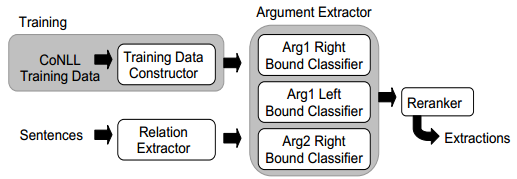
\includegraphics[scale=0.5]{../images/arglearner_architecture.png}
\caption{Proses pelatihan dan ekstraksi \textsc{ArgLearner}}
\label{fig:arglearner_architecture}
\end{figure}

Penelitian berikutnya memperkenalkan \textsc{Ollie} (\textit{Open Language Learning for Information Extraction}) \citep{schmitz2012open} yang menjadikan \textsc{ReVerb} sebagai salah satu modulnya. \textsc{Ollie} menggunakan \textsc{ReVerb} untuk mencari sejumlah (\textit{open pattern})/\textit{template} sebagai panduan untuk mengekstrak \textit{triple} dari kalimat. Perbedaan lain sistem ini dengan pendahulunya adalah relasi yang diekstrak tidak hanya dari kata kerja (\textit{verb}) tetapi bisa juga diekstrak secara implisit dari kata benda (\textit{noun}), kata sifat (\textit{adjective}) \citep{schmitz2012open}. Selain itu \textsc{Ollie} juga menambahkan modul untuk melakukan analisis dan penambahan informasi kontekstual pada hasil ekstraksi sehingga presisi lebih tinggi. Dua modul utama ini diajukan untuk memperbaiki kekurangan dari \textsc{ReVerb} yaitu pembatasan relasi hanya pada kata kerja (\textit{verb}) dan pengabaian konteks kalimat \citep{schmitz2012open}. Proses pelabelan (\textit{labeling}) \textit{dataset} dan ekstraksi \textsc{Ollie} ditunjukkan pada Gambar \ref{fig:ollie_architecture}.

\begin{figure}
\centering
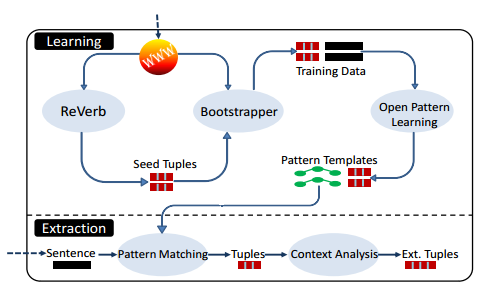
\includegraphics[scale=0.5]{../images/ollie_architecture.png}
\caption{Proses \textit{labeling} dan ekstraksi pada \textsc{Ollie}}
\label{fig:ollie_architecture}
\end{figure}

Salah satu riset terbaru memperkenalkan model sistem \textit{open IE} yang mengganti penggunaan banyak \textit{open pattern}/\textit{template} untuk mengekstrak \textit{triple} pada \textsc{Ollie} \citep{schmitz2012open} dengan hanya enam pola atomik (\textit{atomic patterns}) \citep{angeli2015leveraging}. Enam pola atomik itu digunakan untuk mengekstrak \textit{triple} dari klausa yang \textit{self-contained} dan \textit{maximally compact}. Modul ekstraktor \textit{inter-clauses}, yang menggunakan \textit{multinomial logistic regression classifier}, bertanggungjawab menghasilkan klausa yang \textit{self-contained} (independen secara sintaktik dan semantik), dan modul ekstraktor \textit{intra-clause}, yang menggunakan model \textit{natural logic} \citep{maccartney2007natural}, mengubahnya menjadi klausa yang \textit{maximally compact} (tidak mengandung kata redundan). Model sistem ini diimplementasikan dalam \textsc{Stanford Open IE}, yang merupakan bagian dari kakas NLP \textit{opensource}, \textit{Stanford Core NLP}\footnote{Stanford Core NLP \url{https://stanfordnlp.github.io/CoreNLP/}}.

%-----------------------------------------------------------------------------%
\section{\textit{Open Domain Information Extraction}}
%-----------------------------------------------------------------------------%

\textit{Open domain information extraction} (\textit{open IE}) adalah proses ekstraksi informasi dari dokumen dalam format \textit{triple} $(x, r, y)$ di mana $r$ adalah relasi antara dua buah argumen/entitas $x$ dan $y$ \citep{banko2007open, etzioni2011open}. Relasi pada \textit{triple} diambil dari kata kerja (\textit{verb}) \citep{banko2007open, fader2011identifying} (contoh: kalimat "\textit{Jakarta is the capital of Indonesia}" mengandung \textit{triple} ("Jakarta", "is the capital of", "Indonesia")) atau dari kata lain yang secara implisit merupakan kata kerja \citep{schmitz2012open} (contoh: "\textit{Indonesian President Joko Widodo was born in Surakarta}" mengandung \textit{triple} ("Joko Widodo", "be", "president")). Sedangkan argumen atau entitas yang diekstrak selalu merupakan frase (\textit{noun phrase}) seperti yang juga terlihat di contoh. Format \textit{triple} ini ternyata berlaku umum untuk semua dokumen yang berisi teks bahasa natural sehingga dapat diterapkan pada dokumen dari berbagai domain. Format \textit{triple} yang digunakan \textit{open IE} memiliki kemiripan dengan format yang lazim digunakan pada \textit{knowledge extraction} (KE), yaitu \textit{Resource Data Format} (RDF)\footnote{Resource Data Format W3C \url{https://www.w3.org/RDF/}} \citep{auer2007dbpedia, exner2014refractive}. Namun, perbedaannya adalah \textit{triple} pada \textit{open IE} umumnya tidak mengikuti seluruh spesifikasi RDF dan tidak memiliki himpunan ontologi tetap. Ringkasan perbandingan antara open IE dan KE ditunjukkan pada Tabel \ref{table_paradigm_comparison}. 

\begin{table}
	\centering
	\caption{Perbandingan antara \f{information extraction} tradisional (IE), \f{open domain extraction} (open IE) dan \f{knowledge extraction} (KE)}
	\label{table_paradigm_comparison}
	\begin{tabular}{l c c c}
		\hline 
		\textbf{Aspek} & \textbf{IE} & \textbf{Open IE} & \textbf{KE} \\ 
		\hline 
		\textbf{Domain} & Tertutup & Terbuka & Terbuka \\ 
		\textbf{Format} & Tergantung domain & Triples & RDF Triples \\ 
		\textbf{Ontologi} & Tidak tersedia & Opsional & Wajib \\ 
		\hline 
	\end{tabular} 
\end{table}

Meskipun menggunakan modul dan teknik yang berbeda-beda, model sistem \textit{open IE} umumnya menjalankan proses yang dapat dibagi menjadi tiga langkah/fase \citep{etzioni2011open}:

\begin{enumerate}
	\item Label (\textit{label}): membangun \textit{dataset} untuk \textit{classifier} baik secara manual atau otomatis.
	\item Belajar (\textit{learn}): melatih \textit{classifier} untuk mengekstrak himpunan \textit{triple} dari kalimat menggunakan \textit{dataset} dari fase Label.
	\item Ekstrak (\textit{extract}): mengekstrak himpunan \textit{triple} dari kalimat menggunakan \textit{classifier} yang telah dilatih pada fase Belajar
\end{enumerate}

Hasil ekstraksi \textit{open IE} berguna untuk berbagai \textit{task} seperti \textit{question answering}, \textit{slot filling} \citep{etzioni2011open}, \textit{common sense knowledge acquiring} \citep{singh2002open} dan \textit{information retrieval} \citep{etzioni2011search}. Selain itu, jika dilihat sebagai representasi teks atau dokumen, himpunan \textit{triple} dari \textit{open IE} dapat digunakan sebagai fitur untuk klasifikasi dan \textit{clustering} teks atau dokumen.

%-----------------------------------------------------------------------------%
\section{\textit{Natural Language Processing}}
%-----------------------------------------------------------------------------%

Pemrosesan bahasa natural atau \textit{natural language processing} (NLP) tidak bisa dipisahkan dari information extraction \citep{banko2007open,fader2011identifying,etzioni2011open,angeli2015leveraging}. Semua model sistem \textit{open IE} juga selalu membutuhkan informasi yang dihasilkan oleh \textit{task} NLP seperti \textit{part of speech tagging}, \textit{dependency parsing} dan \textit{named-entity recognition}. Informasi tersebut digunakan sebagai variabel dalam heuristik \textit{open IE} dan juga sebagai fitur untuk \textit{classifier}.

\subsection{\textit{Tokenization}}

\textit{Tokenization} adalah \textit{task} NLP yang bertujuan memotong kalimat atau frase menjadi kata-kata (\textit{tokens}) \citep{manning2008introduction}. Ini merupakan \textit{task} yang paling dasar dan diperlukan sebelum dapat menjalankan \textit{task} lainnya seperti \textit{lemmatization}, \textit{POS tagging}, dsb. Untuk bahasa yang ditulis secara horizontal dan setiap katanya dipisahkan oleh spasi seperti Inggris dan Indonesia, dapat digunakan algoritma berbasis aturan (\textit{rule-based}) yang cukup sederhana \citep{manningptbtokenizer}, yaitu memotong kalimat di antara spasi dan memisahkan tanda baca sebagai \textit{token}. Contoh \textit{tokenization} dari kalimat "Ibu pergi ke pasar." adalah senarai \textit{token} ("Ibu", "pergi", "ke", "pasar", "."). Dalam implementasinya pada bahasa tertentu, algoritma tersebut juga disesuaikan untuk menjalankan proses yang berbeda pada \textit{token} tertentu misalnya gelar atau singkatan yang diikuti titik ("dr.", "Dra.", "Ir.", dsb.).

\subsection{\textit{Part of Speech Tagging}}

\textit{Part of speech} (POS) \textit{tagging} adalah \textit{task} NLP yang bertujuan menentukan \textit{POS tag} atau jenis setiap kata pada kalimat \citep{jurafsky2000speech}. Contoh \textit{POS tag} dasar adalah kata benda (\textit{noun}), kata kerja (\textit{verb}), kata sifat (\textit{adjective}) dst. Gambar \ref{fig:example_pos_tagging} menunjukkan contoh \textit{POS tagging} terhadap kalimat sederhana. \textit{POS tag} dapat digunakan juga oleh \textit{NLP task} yang lain seperti \textit{dependency parsing} dan \textit{named-entity recognition}.

\begin{figure}
	\begin{mdframed}
		\textbf{Input}: "Ibu pergi ke pasar." \\		
		\textbf{Output}: (Ibu, \textit{noun}) (pergi, \textit{verb}) (ke, \textit{preposition}) (pasar, \textit{noun}) (., \textit{punctuation})
	\end{mdframed}
	\caption{Contoh \textit{input} dan \textit{output} \textit{POS tagging}}
	\label{fig:example_pos_tagging}
\end{figure}

Algoritma \textit{POS tagging} umumnya dapat dikelompokkan menjadi dua: berbasis aturan (\textit{rule-based}) dan berbasis stokastik (\textit{stochastic-based}) \citep{jurafsky2000speech}. Salah satu algoritma yang menjadi \textit{state-of-the-art} adalah \textit{maximum-entropy-based POS tagger} (berbasis stokastik) yaitu \textit{tagger} yang mempelajari model probabilitas kondisional \textit{log-linear} (\textit{logistic regression}) menggunakan metode \textit{maximum entropy}.

%\noindent \begin{align}\label{eq:maxent}
%	P(t|h)={\frac 
%		{\exp \left(\sum _{j}\lambda _{j}f_{j}(h,t)\right)}
%		{\sum\limits_{t' \in T} \exp \left(\sum _{j}\lambda _{j}f_{j}(h,t')\right)}
%	}
%\end{align}

\subsection{\textit{Lemmatization}}

\textit{Lemmatization} adalah \textit{task} NLP yang bertujuan mengubah kata imbuhan ke bentuk \textit{lemma} atau bentuk kamus \citep{suhartono2014lemmatization}. Sekalipun memiliki tujuan yang mirip dengan \textit{stemming}, \textit{lemmatization} tidak selalu menghasilkan kata dasar karena menggunakan analisis kosakata dan morfologi yang dapat menghindari terbuangnya \textit{derivational affixes} \citep{manning2008introduction}. Jika dilakukan \textit{stemming} dan \textit{lemmatization} pada \textit{token} "penjahit" maka yang dihasikan sesuai urutan adalah adalah "jahit" dan "penjahit". Hal ini bermanfaat untuk mengurangi terbuangnya informasi yang berguna. Algoritma yang dilaporkan efektif untuk bahasa Indonesia adalah algoritma berbasis aturan penghapusan imbuhan (\textit{affixes}) dan pencarian kamus (\textit{dictionary lookup}) \citep{suhartono2014lemmatization}.

\subsection{\textit{Named-Entity Recognition}}

\textit{Named-entity recognition} (NER) adalah \textit{task} NLP yang mengenali jenis entitas dari \textit{token} pada kalimat. Jenis entitas yang umumnya dikenali contohnya \textit{Person} (nama orang), \textit{Location} (nama lokasi), \textit{Organization} (nama organisasi atau kelompok), dsb. Algoritma \textit{state-of-the-art} untuk NER adalah yang berbasis stokastik seperti \textit{Conditional Random Field} (CRF) dengan fitur-fitur berbasis morfologi, leksikal dan ortografik.

\begin{figure}
	\begin{mdframed}
		\textbf{Input}: "Ibu Budi tinggal di Solo." \\		
		\textbf{Output}: (Ibu) (Budi, \textit{Person}) (tinggal) (di) (Solo, \textit{Location}) (.)
	\end{mdframed}
	\caption{Contoh \textit{input} dan \textit{output} NER}
	\label{fig:example_ner}
\end{figure}

\subsection{\textit{Dependency Parsing}}

\textit{Dependency parsing} adalah \textit{task} NLP yang memetakan dan mengenali pohon hubungan antar \textit{token} dalam kalimat. Masing-masing \textit{token} dapat memiliki satu atau lebih \textit{token} yang bergantung padanya (\textit{dependents}) tapi hanya bisa memiliki satu kepala (\textit{head}) atau tidak memiliki kepala sama sekali. Salah satu algoritma yang menjadi \textit{state-of-the-art} untuk \textit{dependency parsing} adalah algoritma berbasis jaringan syaraf tiruan (\textit{neural network}) yang mempelajari transisi antar \textit{token} \citep{chen2014fast}. 

\subsection{CoNLL-U}

CoNLL-U\footnote{CoNLL-U \url{http://universaldependencies.org/format.html}} adalah format anotasi yang dikembangkan berdasarkan CoNLL-X, format yang disepakati dalam \textit{Conference on Computational Natural Language Learning} ke sepuluh, yang menggunakan himpunan \textit{POS tag} dan \textit{dependency relation} yang berlaku untuk banyak bahasa atau universal \citep{nivre2016universal}. Format \textit{CoNLL-U} ini menggunakan sepuluh buah kolom dengan rincian sebagai berikut:

\begin{enumerate}
	\item ID: Indeks \textit{token} dalam kalimat (mulai dari 1)
	\item FORM: Bentuk asli dari \textit{token}
	\item LEMMA: Bentuk kamus dari \textit{token}
	\item UPOSTAG: \textit{POS tag} universal
	\item XPOSTAG: \textit{POS tag} spesifik untuk bahasa tertentu
	\item FEATS: Fitur tambahan atau spesifik untuk bahasa tertentu
	\item HEAD: ID \textit{token} yang merupaka kepala (\textit{head}) dari \textit{token} ini (0 untuk akar atau \textit{head} kalimat)
	\item DEPREL: \textit{dependency relation} universal
	\item DEPS: \textit{dependency graph} khusus atau spesifik untuk bahasa tertentu
	\item MISC: Anotasi tambahan yang belum tercakup di anotasi lainnya, contoh: \textit{named-entitiy}
\end{enumerate}

Sedangkan himpunan \textit{POS tag} yang dipakai pada CoNLL-U adalah:
\begin{multicols}{2}
	\begin{enumerate}
		\item ADJ: \textit{adjective}
		\item ADP: \textit{adposition}
		\item ADV: \textit{adverb}
		\item AUX: \textit{auxiliary}
		\item CCONJ: \textit{coordinating conjunction}
		\item DET: \textit{determiner}
		\item INTJ: \textit{interjection}
		\item NOUN: \textit{noun}
		\item NUM: \textit{numeral}
		\item PART: \textit{particle}
		\item PRON: \textit{pronoun}
		\item PROPN: \textit{proper noun}
		\item PUNCT: \textit{punctuation}
		\item SCONJ: \textit{subordinating conjunction}
		\item SYM: \textit{symbol}
		\item VERB: \textit{verb}
		\item X: \textit{other}
	\end{enumerate}
\end{multicols}

Sementara himpunan \textit{dependency relation} yang dipakai adalah:

\begin{multicols}{2}
	\begin{enumerate}
		\item acl: \textit{clausal modifier of noun (adjectival clause)}
		\item advcl: \textit{adverbial clause modifier}
		\item advmod: \textit{adverbial modifier}
		\item amod: \textit{adjectival modifier}
		\item appos: \textit{appositional modifier}
		\item aux: \textit{auxiliary}
		\item case: \textit{case marking}
		\item cc: \textit{coordinating conjunction}
		\item ccomp: \textit{clausal complement}
		\item clf: \textit{classifier}
		\item compound: \textit{compound}
		\item conj: \textit{conjunct}
		\item cop: \textit{copula}
		\item csubj: \textit{clausal subject}
		\item dep: \textit{unspecified dependency}
		\item det: \textit{determiner}
		\item discourse: \textit{discourse element}
		\item dislocated: \textit{dislocated elements}
		\item expl: \textit{expletive}
		\item fixed: \textit{fixed multiword expression}
		\item flat: \textit{flat multiword expression}
		\item goeswith: \textit{goes with}
		\item iobj: \textit{indirect object}
		\item list: \textit{list}
		\item mark: \textit{marker}
		\item nmod: \textit{nominal modifier}
		\item nsubj: \textit{nominal subject}
		\item nummod: \textit{numeric modifier}
		\item obj: \textit{object}
		\item obl: \textit{oblique nominal}
		\item orphan: \textit{orphan}
		\item parataxis: \textit{parataxis}
		\item punct: \textit{punctuation}
		\item reparandum: \textit{overridden disfluency}
		\item root: \textit{root}
		\item vocative: \textit{vocative}
		\item xcomp: \textit{open clausal complement}
	\end{enumerate}
\end{multicols}

%-----------------------------------------------------------------------------%
\section{\textit{Supervised Learning}}
%-----------------------------------------------------------------------------%

\textit{Supervised learning} adalah teknik \textit{machine learning} yang mempelajari pola dari \textit{dataset} yang telah diberi label atau dikelompokkan \citep{mohri2012foundations}. Metode \textit{supervised learning} dapat dibagi menjadi dua, yaitu deskriptif (\textit{descriptive learning}) dan generatif (\textit{generative learning}). Pada \textit{descriptive learning} mencari fungsi untuk memetakan data $x$ ke label $y$ atau probabilitas posterior (\textit{posterior probability}) $p(y|x)$ (contoh: \textit{logistic regression}, \textit{support vector machine}, \textit{multi-layer perceptron}, dsb.) sedangkan \textit{generative learning} mencari probabilitas gabungan (\textit{joint probability}) $p(x,y)$ lebih dulu sebelum menggunakan \textit{Bayes Rules} untuk menghitung $p(y|x)$ (contoh: \textit{naive bayes classifier}, \textit{decision tree}, dsb.) \citep{ng2002discriminative}. Penelitian ini membandingkan empat buah model klasifikasi biner yang dihasilkan oleh metode-metode berikut:

\subsection{\textit{Logistic Regression}}

\textit{Logistic regression} adalah metode pemodelan deskriptif yang mencari fungsi hipotesis yang memetakan data $x$ ke kelas $y$ yang dapat dipisahkan fungsi logistik/\textit{sigmoid} (\ref{eq:logistic_function}) sesuai kelasnya $\{0,1\}$ \citep{theodoridis2015machine} seperti visualisasi pada Gambar \ref{fig:logreg}. Fungsi hipotesis dihasilkan dengan mencari bobot $\theta$ yang dapat meminimumkan \textit{cost function} (\ref{eq:logreg_cost_function}) menggunakan algoritma \textit{gradient descent}.

\begin{figure}
\centering
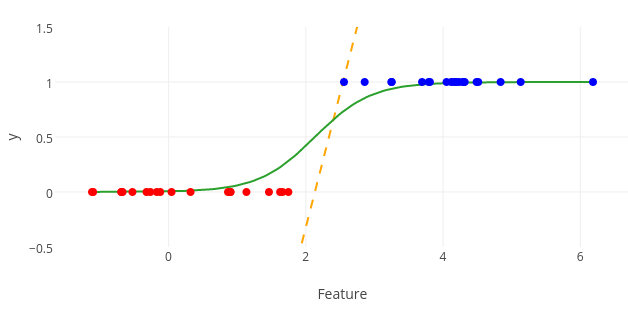
\includegraphics[scale=0.5]{../images/logreg.png}
\caption{Contoh hasil pemetaan (titik merah dan biru) fungsi \textit{logistic regression} dari fitur $x$ ke kelas $y$ yang dapat dipisahkan oleh fungsi logistik/\textit{sigmoid} (garis hijau) (sumber: \url{https://florianhartl.com})}
\label{fig:logreg}
\end{figure}


\noindent \begin{align}\label{eq:logistic_function}
	\sigma(t) = {\frac {1}{1+e^{-t}}} \\[0.2cm]
	\textrm{di mana $t$ adalah fungsi hipotesis, } t = \theta^{T}x \nonumber 
\end{align}

\noindent \begin{align}\label{eq:logreg_cost_function}
	L(\theta) = - \sum_{n=1}^{N} \, (y_{n} \ln \sigma(t) \, + \, (1 - y_{n}) \ln (1 - \sigma(t)))
\end{align}

\noindent \begin{align}\label{eq:gradient_descent}
	\theta_{j} &= \theta_{j} - \alpha \frac{\partial}{\partial \theta_{j}} L(\theta) \\ \nonumber 
	di mana, \theta &= \textrm{bobot} \\ \nonumber 
			 \alpha &= \textit{learning rate} \\ \nonumber 		 
\end{align}


\subsection{\textit{Support Vector Machine}}

\textit{Support vector machine} (SVM) merupakan pemodelan yang mencari fungsi \textit{hyperplane} yang memisahkan data sesuai kelasnya dengan menggunakan \textit{decision boundary} yang memiliki jarak optimal dengan \textit{hyperplane} \citep{theodoridis2015machine} seperti pada Gambar \ref{fig:svm}. Untuk memisahkan data yang tidak terpisahkan secara linier (\textit{non-linearly separable}), dapat digunakan fungsi \textit{kernel} untuk memetakan data sehingga bisa bisa dipisahkan secara linier. Salah satu fungsi \textit{kernel} yang umum digunakan pada \textit{task} NLP adalah \textit{kernel} polinomial (\ref{eq:poly_kernel}) \citep{joachims1998text}.

\begin{figure}
\centering
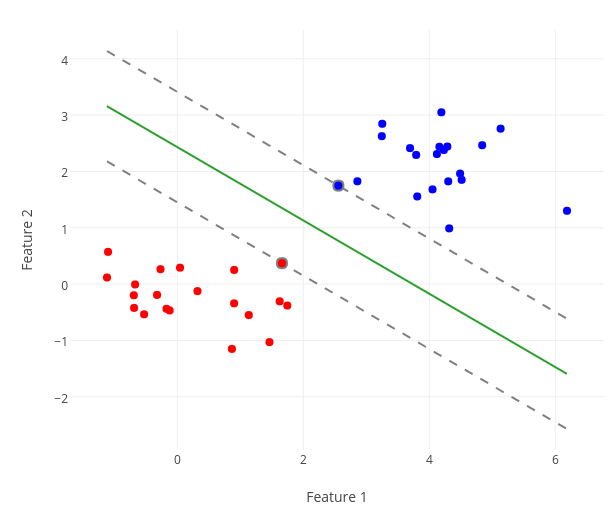
\includegraphics[scale=0.5]{../images/svm.png}
\caption{Contoh fungsi linier (garis hijau) dari SVM yang memisahkan dua kelompok data dua dimensi (titik merah dan biru) menggunakan dua \textit{support vector} (sumber: \url{https://florianhartl.com})}
\label{fig:svm}
\end{figure}

\noindent \begin{align} \label{eq:poly_kernel}
K(x,y) &= (x^\mathsf{T} y + c)^{d} \\ \nonumber
\textrm{di mana, } x &= \textrm{data atau fitur, } \\ \nonumber 
	y &= \textrm{kelas atau label, } \\ \nonumber
	d &= \textrm{derajat polinomial, } \\ \nonumber 
	c &= \textrm{konstanta} \\ \nonumber 
\end{align}

%\noindent \begin{align} \label{eq:cost_function}
%f(c_{1}\ldots c_{n}) &= \sum _{i=1}^{n}c_{i}-{\frac {1}{2}}\sum _{i=1}^{n}\sum _{j=1}^{n}y_{i} \, c_{i} \, K({\vec {x}}_{i},{\vec {x}}_{j})y_{j}c_{j} \\ \nonumber 
%& \text{di mana, } \sum _{i=1}^{n}c_{i}y_{i} = 0,\,\text{dan }0\leq c_{i}\leq {\frac {1}{2n\lambda }}\; \text{untuk semua }i. \\ \nonumber 
%\end{align}

\subsection{\textit{Multi-Layer Perceptron}}

\textit{Multi-Layer Perceptron} (MLP) atau \textit{feed-forward neural network} adalah pemodelan klasifikasi nonlinier berbasiskan jaringan syaraf tiruan (\textit{perceptron}) yang memiliki lebih dari satu \textit{hidden layer} yang berisi sejumlah neuron \citep{theodoridis2015machine} seperti yang divisualisasikan pada Gambar \ref{fig:mlp}. Nilai \textit{output} dari suatu neuron ditentukan oleh \textit{input} $x$, bobot (\textit{weight}) $w$, \textit{bias} $b$ dan fungsi aktivasi $f$, $o(\vec{x}) = f(\vec{w} \cdot \vec{x} + \vec{b})$ \citep{mitchell1997machine}. Contoh fungsi aktivasi yang bisa digunakan \citep{mitchell1997machine} adalah:

\begin{enumerate}
	\item Fungsi \textit{sign} : $ f(x) = 1 \; \textrm{if} \; x > 0 \; \textrm{selain itu} -1 $
	\item Fungsi \textit{sigmoid/logistic} : $ f(x)={\frac {1}{1+e^{-x}}} $
	\item Fungsi \textit{tanh}: $ f(x)=\tanh(x)={\frac {2}{1+e^{-2x}}}-1 $
	\item Fungsi \textit{rectifier}: $ f(x)=\max(0,x) \citep{nair2010rectified} $
\end{enumerate}

MLP dilatih dengan menyesuaikan bobot secara iteratif menggunakan algoritma \textit{gradient descent} dan \textit{backpropagation} \citep{theodoridis2015machine}.

\begin{figure}
\centering
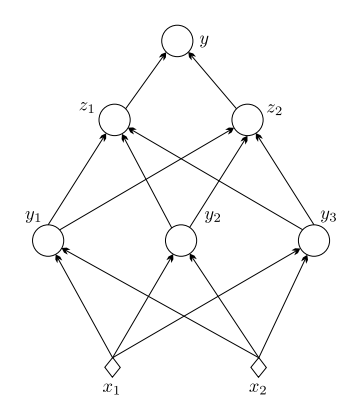
\includegraphics[scale=0.5]{../images/mlp.png}
\caption{Visualisasi MLP dengan \textit{input layer} \{$x_1, x_2$\}, dua \textit{hidden layer} \{\{$y_1, y_2, y_3$\}, \{$z_1, z_2$\}\} dan satu \textit{output layer} \{$y$\} (sumber: \cite{theodoridis2015machine})}
\label{fig:mlp}
\end{figure}

\subsection{\textit{Random Forest}}

\textit{Random forest} adalah metode \textit{bagging} lebih dari satu varian \textit{decision tree} (\textit{forest}) dengan pemilihan fitur yang acak (\textit{random}) \citep{breiman2001random}. \textit{Bagging} sendiri adalah metode klasifikasi berdasarkan voting lebih dari satu varian \textit{classifier} dengan tujuan meningkatkan kemampuan generalisasi \citep{breiman1996bagging}. Sedangkan \textit{decision tree} adalah pemodelan klasifikasi generatif yang membangun serangkaian tes terhadap data/fitur untuk menolak kemungkinan kelas sampai hanya tersisa satu kelas \citep{theodoridis2015machine}. Visualisi \textit{random forest} ditunjukkan pada Gambar \ref{fig:random-forest}.

\begin{figure}
\centering
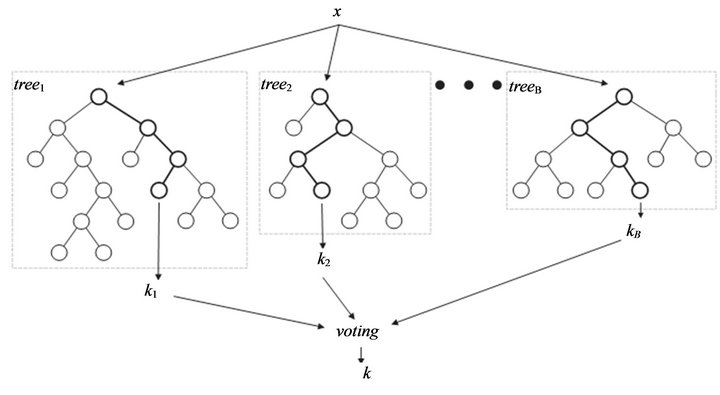
\includegraphics[scale=0.5]{../images/random-forest.png}
\caption{Visualisasi \textit{random forest} yang memprediksi kelas $k$ untuk data $x$ berdasarkan voting hasil klasifikasi setiap \textit{tree} $\{k_1, k_2, .., k_b\}$ (sumber: \url{http://wwww.scirp.org})}
\label{fig:random-forest}
\end{figure}
